\chapter{NORUMIS - Nonmonotonic Rule Mining System}\label{sec:meth}

\section{System Overview}

\begin{figure}[ht]
\centering
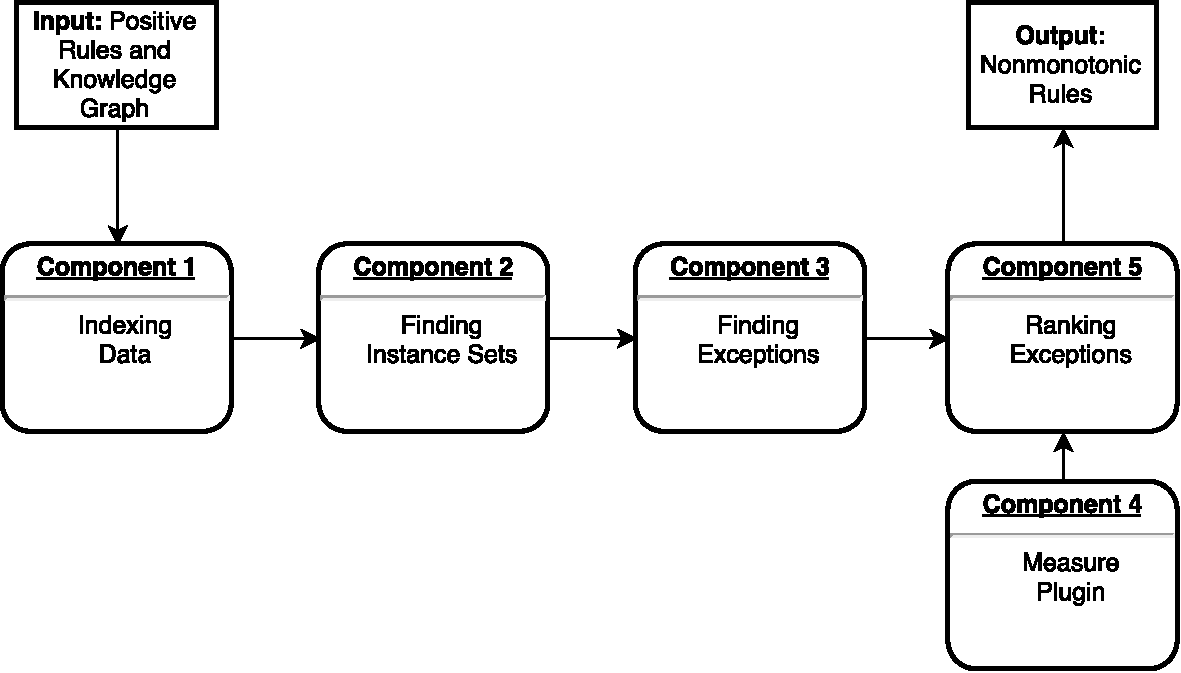
\includegraphics[width=0.85\textwidth]{figures/system_overview}
\caption{Overview of Our System}
\label{rdf}
\end{figure}

\section{Steps in the System}

Our methodology for solving the QHTR problem comprises four steps, which we now discuss in details.
%\begin {enumerate*} [label=(\itshape\roman*\upshape)]
%\item[(1)] determining $r$-normal and $r$-abnormal substitutions for every rule $r\in \cR_{H}$,
%\item[(2)] computing exception witness sets $\mi{EWS(r,\cG, X)}$, $\mi{EWS(r,\cG,Y)}$ and $\mi{EWS(r,\cG,X,Y)}$ for $r$ with $h(X,Y)$ in the head,
%\item[(3)] construction of rule revisions,
%\item[(4)] step-wise exception ranking and combining the results.
%\end {enumerate*} 
%We now discuss these steps in more details. 
\medskip

\noindent \textbf{Step 1.} After mining Horn rules using a state-of-the-art algorithm (e.g., \cite{newrulemine} or \cite{amieplus}), we compute for each rule $r$ the $r$-\emph{normal} and $r$-\emph{abnormal} substitutions.
\medskip


\noindent \textbf{Step 2 and 3.} Then for every rule $r\in \cR_H$ with the head atom $\mi{h(X,Y)}$ we determine three $\mi{EWS}$ sets: $\mi{EWS(r,\cG,X)}$, $\mi{EWS(r,\cG,Y)}$ and $\mi{EWS(r,\cG,\tuple{X,Y})}$. From the obtained $\mi{EWS}$s we create $|\mi{EWS(r,\cG,X)}|+|\mi{EWS(r,\cG,Y)}|+|\mi{EWS(r,\cG,\tuple{X,Y})}|$ potential revisions by adding every determined exception in the form of a negated atom to the rule $r$ at hand.
\medskip

\noindent \textbf{Steps 4.} 
After all candidate revisions are constructed we rank them and determine the resulting set $\cR_{\mi{NM}}$ by selecting for every rule the revision that is ranked the highest.

To find such globally best revised ruleset $\cR_{\mi{NM}}$ too many candidate combinations have to be checked, which is impractical due to the large size of the KG $\cG$ and $\mi{EWS}$s. 

Thus, instead we incrementally build $\cR_{\mi{NM}}$ by considering every $r_i \in \cR_{H}$ and choosing the locally best revision $r_i^{j}$ for it.
For that we exploit three ranking functions: a naive one and two more sophisticated ones, which invoke the novel concept of \emph{partial materialization} (\textbf{\em PM}). Intuitively, the idea behind it is to rank candidate revisions not based on $\cG$, but rather on its extension with predictions produced by other (selectively chosen) rules (grouped into a set $\cR'$), thus ensuring a cross-talk between the rules. We now describe the ranking functions in more details.

\begin{itemize}
\item {\textbf{\em Naive (N)}} ranker is the most simple function, which prefers the revision $\mi{r^j_i}$ with the highest value of $\mi{rm(r^j_{i},\cG)}$ among all revisions of $r_i$.
\smallskip

\item {\textbf{\em PM}} ranking function prefers $\mi{r^j_i}$ with the highest value of
\begin{equation}
\label{pm}
score(r^j_i,\cG)=\dfrac{\mi{rm(r^j_i,\cG_{\cR'})+rm({r^j_i}^{aux},\cG_{\cR'})}}{2}
\end{equation}
 where $\cR'$ is the set of rules $r_k'$, which are rules from $\cR_H\backslash r_i$ with all candidate exceptions for $r_k$ incorporated at once. Informally, $\cG_{\cR'}$ contains only facts that can be safely predicted by the rules from $\mi{\cR_H\backslash r_i}$, i.e., there is no evident reason (candidate exceptions) for avoiding predictions of these facts.
 \smallskip
 
\item {\textbf{\em OPM}} is similar to \textbf{{\em PM}}, but the selected ruleset $\cR'$ contains only those rules whose Horn version appears above the considered rule $r_i$ in the ruleset $\cR_H$, ordered (\textbf{\em O}) based on some chosen measure (e.g., the same as $\mi{rm}$). 
\end{itemize}

The algorithms for Step 1 and 2 are extended versions of those from \cite{iswc2016}. We neglect further details here for space reasons.
%\ju{(General comment) From my understanding of this section, one problem that I see is that you do not distinguish revisions based on the number of variables in the EWS. In other words, EWS(r,G,X) and EWS(r,G,<X,Y>) are considererd equally. My feeling is that EWS with the smaller number of variables will score higher because it will be easier to find evidence (ie. support and number of comflicts) that support such EWS. For this paper this is obviously fine, but in the future I think more sophisticated ranking functions must be devised.} DS: sure, this is also among my concerns. As you rightly mentioned, the choice of the best revision needs more involved rankers. We treated exceptions in all EWS equally just for this preliminary results.

\section{Implementation}

\section{Scalability}